\documentclass[
	12pt,
	a4paper,
	pdftex,
	czech,
	titlepage
]{report}

\usepackage[czech]{babel}
\usepackage[utf8]{inputenc}
\usepackage{lmodern}
\usepackage{textcomp}
\usepackage[T1]{fontenc}
\usepackage{amsfonts}
\usepackage{titlesec}
\usepackage{graphicx}

\titleformat{\chapter}
{\normalfont\LARGE\bfseries}{\thechapter}{1em}{}
\titlespacing*{\chapter}{0pt}{0ex plus 1ex minus .2ex}{2.0ex plus .2ex}

\begin{document}

\begin{titlepage}
	\vspace*{-2cm}
	{\centering
\includegraphics[scale=1.0]{logo.pdf}\par}
	\centering
	\vspace*{2cm}
	{\Large Semestrální práce z KIV/WEB\par}
	\vspace{1.5cm}
	{\Huge\bfseries Konferenční systém\par}
	\vspace{2cm}

	{\Large Jiří Velek\par}
	{\Large A20B0269P\par}
	{\Large jvelek@students.zcu.cz\par}

	\vfill

	{\Large 18.\,12.\,2021}
\end{titlepage}

\tableofcontents
\thispagestyle{empty}
\clearpage

\chapter{Popis webové aplikace}
\setcounter{page}{1}
Webová aplikace slouží k publikaci článků a jejich popisu. Každý registrovaný
uživatel může publikovat vlastní články. Po přidání článku autor čeká na
recenzenty, aby napsali recenzi. Tu si poté přečtou administrátoři a po jejím
vyhodnocení se rozhodnou, zda článek schválí, nebo odstraní.
Pří schválení administrátorem se články zobrazí i ostatním uživatelům.
Uživatelé mohou
vyhledávat články podle jejich názvu, nebo podle uživatele, který ho napsal.

\chapter{Popis databáze}
Databáze obsahuje celkem 4 tabulky: role uživatelů, uživatele, články a recenze
článků.

\begin{center}

	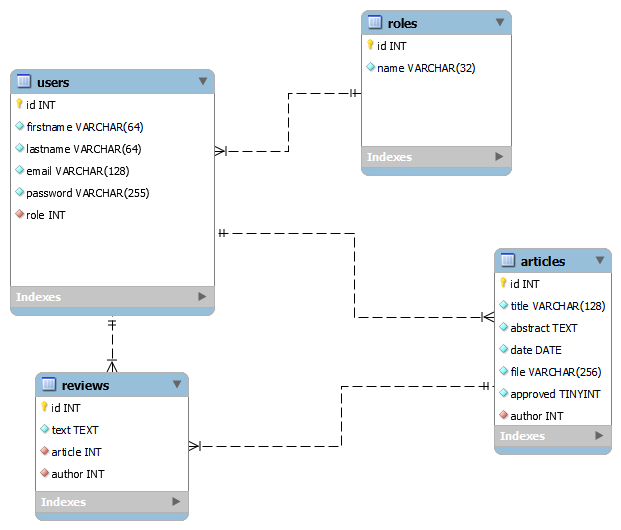
\includegraphics[width=\textwidth,height=\textheight,keepaspectratio]{semestralka_model}
	ERA model databáze
\end{center}

\section{Role uživatelů}
Tabulka role uživatelů obsahuje pouze dva sloupečky --- id role a název role,
tato tabulka určuje, kam mohou uživatelé s danou rolí přistupovat a co na webu
mohou ovládat.

\section{Uživatelé}
Tabulka uživatelů obsahuje id uživatele, jméno, přijmení, e-mail, zašifrované
heslo a roli uživatele. Popisuje jednotlivé uživatele a jejich pravomoce na
webu (podle jejich role).

\section{Články}
Tabulka článků drží informace o jednotlivých článcích --- id článku, autor,
abstrakt,
datum přidání článku, odkaz na přiložený PDF soubor, informace o tom, zda byl
článek schválen.

\section{Recenze}
Tabulka recenzí obsahuje id recenze, autora recenze, id článku, ke kterému
recenze patří a samotný text recenze.

\chapter{Využité technologie}
Web je napsán v PHP verzi 8.1. Celý web využívá MVC architekturu. Vrstva view
je
realizována pomocí knihovny Twig. Samotný vzhled webu je řešen pomocí
bootstrapu verze 5.

\chapter{Uživatelská příručka}

\section{Hlavní stránka}
Hlavní stránka popisuje web a jeho obsah.

\section{Články}
Stránka článků obsahuje seznam všech přidaných a akceptovaných článků. Po
rozkliknutí článku je uživatel přesměrován na stránku se samotným článkem, kde
si může přečíst celý abstrakt a stáhnout přiložený PDF soubor.

\section{Přidávání článků}
K přidání nového článku je třeba být přihlášen, uživatel vyplní titulek článku,
abstrakt a přiloží PDF soubor. Poté už jen čeká na recenzi od recenzenta a
schválení administrátorem.

\chapter{Závěr}
Práce na webové aplikaci byla zajímavá. Ukázala, že napsat i velmi jednoduchý
web může být docela náročné, a proto se dnes využívá různá řada technologií,
které vývoj webu usnadňují.

\end{document}